

\section{Tracking}
\label{Sect:Tracking}

The MICE instrumentation allowed individual particles to be tracked from TOF0 to
the EMR, a distance of more than 15\,m.
High-resolution particle tracking was provided by two
scintillating-fibre trackers (section~\ref{SubSect:Tracker}).
The precise relative alignment of the time-of-flight hodoscopes and
the trackers was obtained by combining the measurements of both
detector systems (section~\ref{SubSect:DA}). 

\graphicspath{{06-Tracking/Figures/}}

\subsection{Trackers}
\label{SubSect:Tracker}

The two high-precision scintillating-fibre trackers each had a
sensitive volume that was 110\,cm in length and 30\,cm in
diameter~\cite{Ellis:2010bb}.
Each tracker was composed of five stations (labelled 1 to 5, with
station 1 being closest to the cooling cell) held in position using a
carbon-fibre space-frame.  
Adjacent stations were separated by different distances ranging from
20\,cm to 35\,cm.
The separations were chosen to ensure that the azimuthal rotation of
track position did not repeat from one station to the next.
This property was exploited in the ambiguity-resolution phase of the
pattern recognition.
Each tracker was instrumented with an internal LED calibration system
and four 3-axis Hall probes to monitor the field.
A photograph of one of the trackers on the bed of the coordinate
measuring machine used to verify the mechanical alignment of the
stations is shown in figure~\ref{Figure:FullTracker}.
\begin{figure}
  \begin{center}
    \includegraphics[width=0.6\textwidth,keepaspectratio=true,]{FullTracker.png}
  \end{center}
  \caption{
    Photograph, with UV-filtered light, of one of the MICE trackers, showing the five stations.
    Each station has three doublet planes of scintillating fibres, each plane
    at 120$^\circ$ to the next (the central fibres of each plane can
    be seen as darker lines traversing the station).
    %Bundles of seven 350\,$\mu$m fibres were grouped together, to be read out by 1\,mm light guides.
  }
  \label{Figure:FullTracker}
\end{figure}

Each tracker station consisted of three doublet layers of 350\,$\mu$m
scintillating fibres; these layers were arranged such that each was
set at an angle of 120$^\circ$ with respect to the next.
This arrangement ensured that there were no inactive regions between
adjacent fibres.
Fibres were grouped into one bundle of seven for each readout
channel, to match the resolution to that imposed by multiple
scattering and reduce the overall number of readout channels.
This resulted in a spatial resolution per doublet layer of 470\,$\mu$m
and a measured light yield of approximately 10
photo-electrons~\cite{Ellis:2010bb}.
The light from the seven scintillating fibres was coupled into a
single clear fibre which took it to a visible light photon counter
(VLPC)~\cite{VLPC}.
The signals from the VLPCs were digitised using electronics developed
by the D0 collaboration~\cite{Abazov:2005pn}. \\

\noindent\textbf{Reconstruction} \\
\noindent
The reconstruction software for the trackers is described
in~\cite{Dobbs:2016ejn}.
Each of the 15 doublet layers provided 214 readout channels.
Calibration data taken without beam was used to determine the pedestal and the gain of each channel.
These calibrations were used to correct the number of photoelectrons
(NPE) corresponding to the signal recorded by the tracker
electronics.
The first step in the reconstruction was to record the unique channel
number associated with each NPE value in a ``digit''.
Digit profiles were used to identify hot or dead channels which
were masked from the reconstruction to reduce the rate of ambiguities
that had to be resolved in the pattern recognition and to ensure the
accuracy of the calibration.
The reconstruction proceeded to create ``spacepoints'' from the
intersection of digits in adjacent doublet layers.
Spacepoints were constructed from clusters from all three planes (a
triplet spacepoint) or from any two out of the three planes (a doublet
spacepoint).
The pattern-recognition algorithm searched for spacepoints from
neighbouring stations that were consistent with the helical trajectory
of a charged particle in the solenoidal field.
In the final stage of the tracker reconstruction the track parameters
were estimated using a Kalman filter. \\

\newpage

\noindent\textbf{Noise}\\
\noindent
Digits above a certain NPE threshold were admitted to the
spacepoint-finding algorithm.
Noise in the electronics arising from, for example, the thermal
emission of electrons, could give rise to digits passing the threshold.
Any digit not caused by the passage of a charged particle was
classified as noise.
To isolate noise from signal during beam-on data collection, events
containing a track which included a spacepoint in each of the five
tracker stations were selected.
All digits corresponding to the track were removed from the total set
of digits and the remainder were considered to be noise.
The average noise rate per channel per event was then calculated as
the total number of digits above the NPE threshold divided by the
number of active channels and the  number of events in the sample.
The result of this calculation was that, for an NPE threshold of 2,
the fraction of digits arising from noise was 0.18\% in the upstream
tracker and 0.06\% in the downstream tracker. \\

\noindent\textbf{Track-finding efficiency} \\
\label{trackers:performance:efficiency}
\noindent
The track-finding efficiency was determined using a sample of events
for which the time-of-flight determined from hits in TOF1 and
TOF2 was consistent with passage of a muon.
This requirement ensured that the particle had been transmitted
successfully through the magnetic channel, crossing both trackers.
The track-finding efficiency was defined to be the number of
events in which a track was successfully reconstructed divided by the
total number of events in the sample.
The results of the efficiency analysis are tabulated in
table~\ref{Table:tracker_efficiency_results} for a range of nominal
beam momentum and emittance settings.
The track-finding efficiency obtained in this way averaged over
beam conditions was 98.70\% for the upstream tracker and 98.93\%
for the downstream tracker.
The spacepoint-finding efficiency, defined as the number of
spacepoints found divided by the number of space points expected, was
also determined.
The spacepoint-finding efficiency is summarised for a range of beam
conditions in
table~\ref{Table:tracker_spacepoint_efficiency_results}.
%Overall the high track-finding efficiency was found to be consistent
%with that introduced by the number of dead channels and did not
%introduce significant systematic uncertainties in analysis of the
%MICE data.
\begin{table}
  \caption{
    The track finding efficiency for the upstream and downstream
    trackers for 140\,MeV/$c$ and 200\,MeV/$c$ beams, and for 3, 6 and
    10\,mm nominal emittances.}
  \begin{center}
    \begin{tabular}{| c | c | c | c |}
      \hline 
      \textbf{Momentum} & \textbf{Emittance} & \textbf{Upstream tracks found} & \textbf{Downstream tracks found} \\ \hline
        200 MeV/$c$ & 3\,mm  & 98.38\% & 99.19\% \\ %H36aa
        200 MeV/$c$ & 6\,mm  & 99.42\% & 96.07\% \\ %H25c 
        140 MeV/$c$ & 6\,mm  & 98.37\% & 99.16\% \\ %H36c
        140 MeV/$c$ & 10\,mm & 98.47\% & 98.93\% \\ \hline %H36d
        \multicolumn{2}{| c |}{Average} & 98.70\% & 98.21\% \\
        \hline
    \end{tabular}
  \end{center}
  \label{Table:tracker_efficiency_results}
\end{table}
\begin{table}
  \caption{
    The spacepoint-finding efficiency, in the presence of a
    track, for the upstream and downstream trackers for 140\,MeV/$c$
    and 200\,MeV/$c$ beams, and for 3, 6 and 10\,mm nominal
    emittances.  }
  \begin{center}
    \begin{tabular}{| c | c | c | c |}
      \hline
      \textbf{Momentum} & \textbf{Emittance} & \textbf{Upstream spacepoints found} & \textbf{Downstream spacepoints found} \\ \hline
        200 MeV/$c$ & 3\,mm  & 98.04\% & 97.41\% \\ %H36aa
        200 MeV/$c$ & 6\,mm  & 99.41\% & 94.63\% \\ %H25c 
        140 MeV/$c$ & 6\,mm  & 97.99\% & 99.16\% \\ %H36c
        140 MeV/$c$ & 10\,mm & 98.07\% & 97.44\% \\ \hline %H36d
        \multicolumn{2}{| c |}{Average} & 98.44\% & 97.01\% \\
        \hline
    \end{tabular}
  \end{center}
  \label{Table:tracker_spacepoint_efficiency_results}
\end{table}

The efficiency of the trackers over the data taking period was
evaluated by selecting events with a measured time-of-flight between
TOF1 and TOF2 consistent with the passage of a muon.
Events were required to contain at least one hit within the fiducial
volume of the tracker.
An event was added to the numerator of the efficiency calculation if
it contained a single space point in each of the five tracker
stations.
The evolution of the tracking efficiency in the upstream and
downstream trackers is shown in
figure~\ref{fig:trackers:performance:historical}.
The efficiency is shown separately for data taken in the presence of a
magnetic field (``helical'') and with the solenoids turned off
(``straight'').
The data shows that the efficiency was generally greater than 99.0\%.
Water vapour ingress to the cold end of the VLPC cassettes caused the loss of
channels and contributed to a reduction in the tracking efficiency.
This was recovered by warming and drying the VLPCs. \\
\begin{figure}[htb]
  \begin{center}
    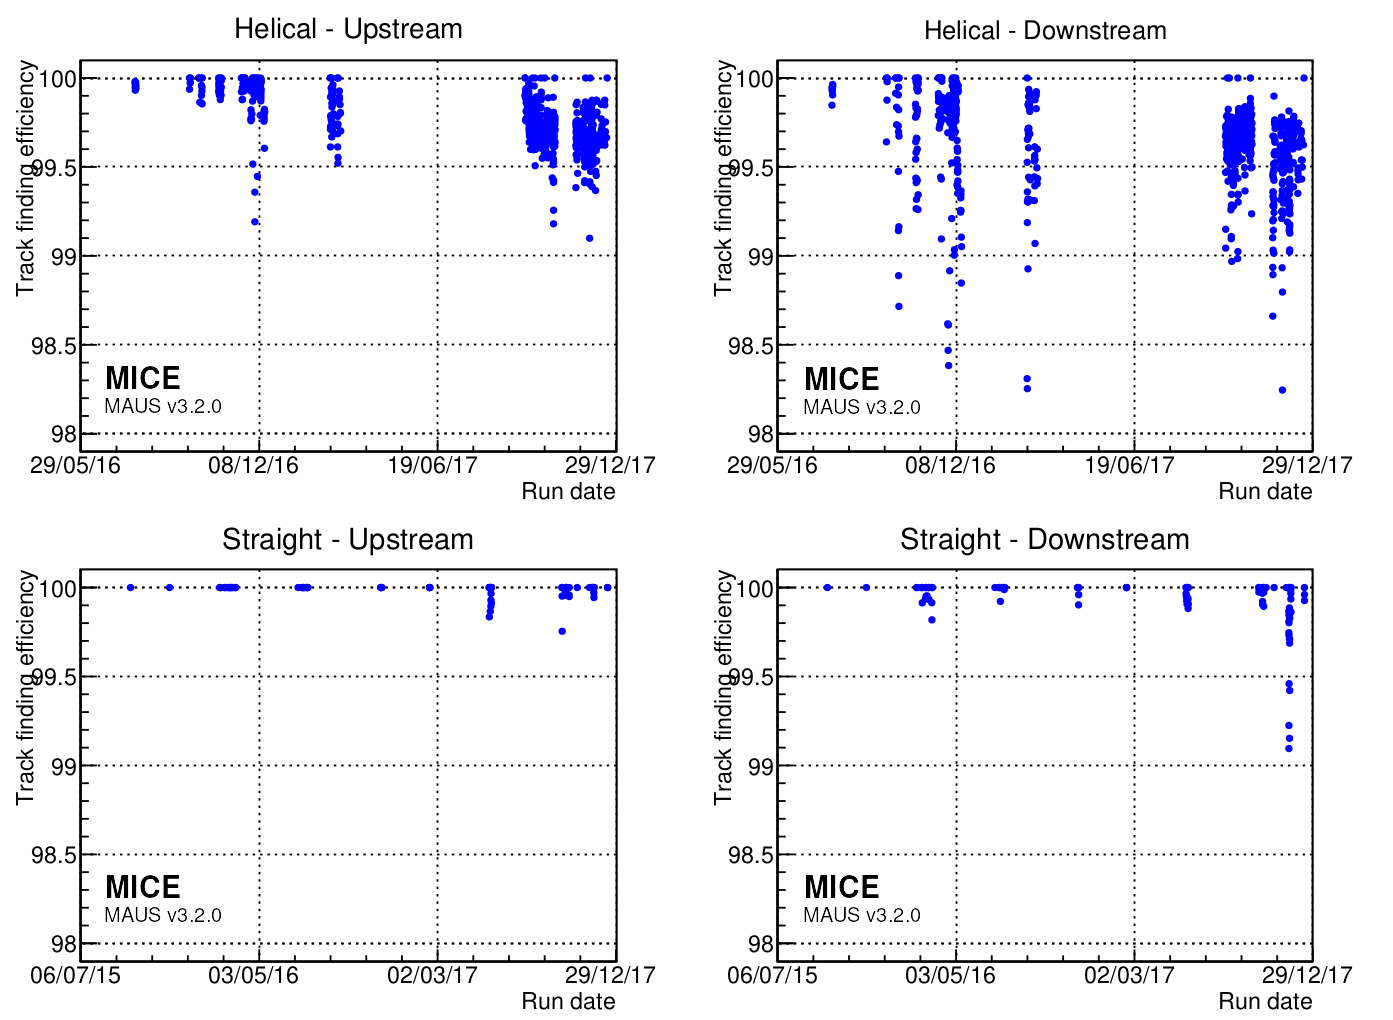
\includegraphics[width=0.90\textwidth]{historical_analysis_plot_logo.png}
  \end{center}
  \caption{
    Evolution of the straight and helical track finding efficiencies
    over time for: the upstream (left); and downstream (right) trackers
    during the key periods of data taking since 2015.
    Each dot represents a single data taking run between 10 minutes and 3 hours long.
  }
  \label{fig:trackers:performance:historical} 
\end{figure}

\noindent\textbf{Track-fit performance} \\
\noindent
Monte Carlo simulation with realistic field, beam conditions and detectors geometry was used to estimate the performance of the track fit.
A beam centred at 140\,MeV/$c$ with 10\,mm nominal emittance,
representing a typical data set, was used for the study.
Results are presented in
figure~\ref{trackers:performance:resolutions:up} for the upstream
tracker and figure~\ref{trackers:performance:resolutions:down} for the
downstream tracker.
The resolution in the total momentum and transverse momentum is
observed to be $\sim1.1$\,MeV/$c$ independent of momentum in the range
120\,MeV/$c$ to 160\,MeV/$c$.
%The small bias in reconstructed momentum and transverse momentum is {\color{red} understood to be due to ...?}
The small bias in the transverse and the total momentum did not give rise to significant effects in the analysis and was considered in systematic error studies.
\begin{figure}[htb]
  \begin{center}
    \begin{tabular}{cc}
      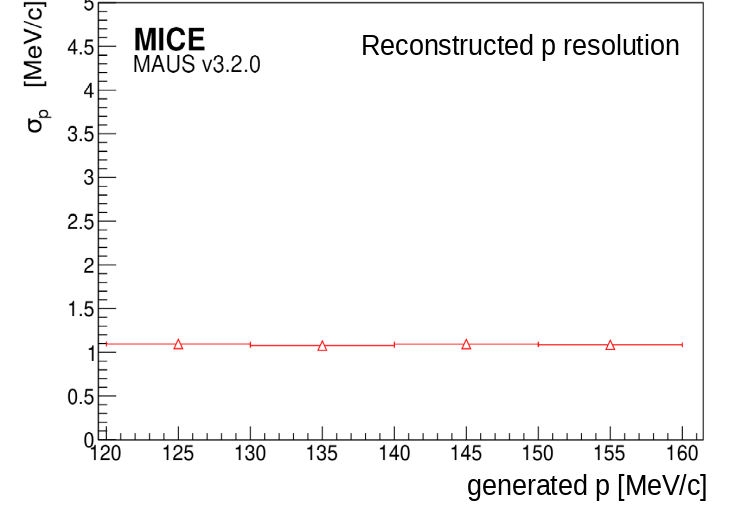
\includegraphics[width=0.49\textwidth]{upstream_p_resolution_p_logo.png} &	
      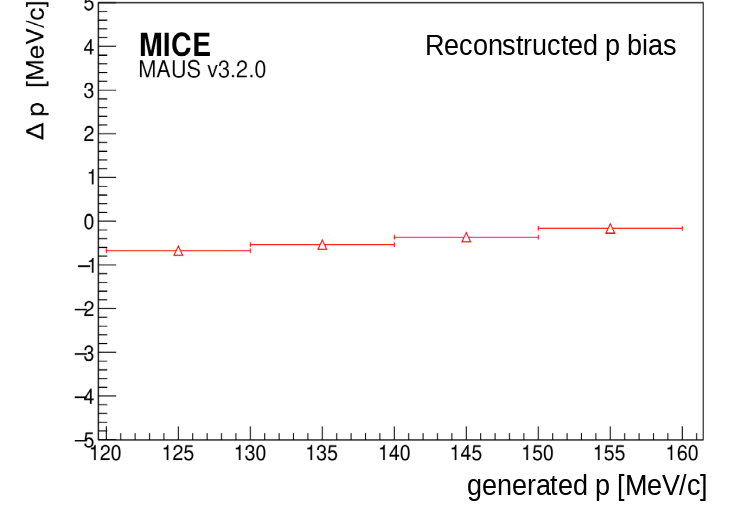
\includegraphics[width=0.49\textwidth]{upstream_p_bias_p_logo.png} \\
      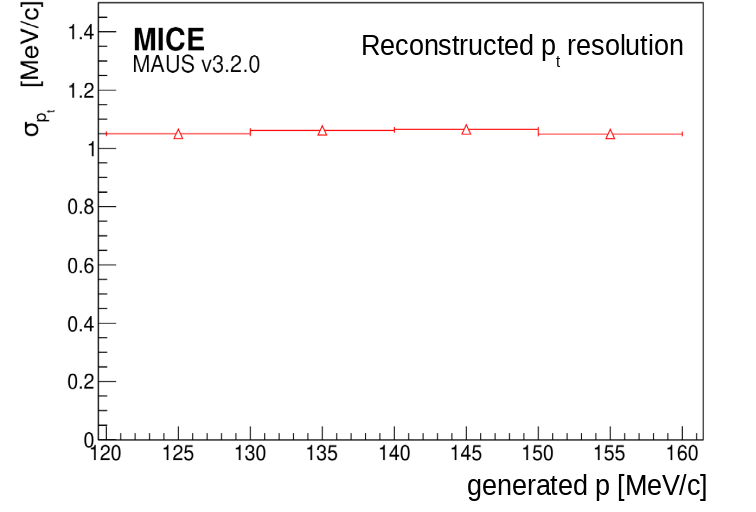
\includegraphics[width=0.49\textwidth]{upstream_pt_resolution_p_logo.png} &
      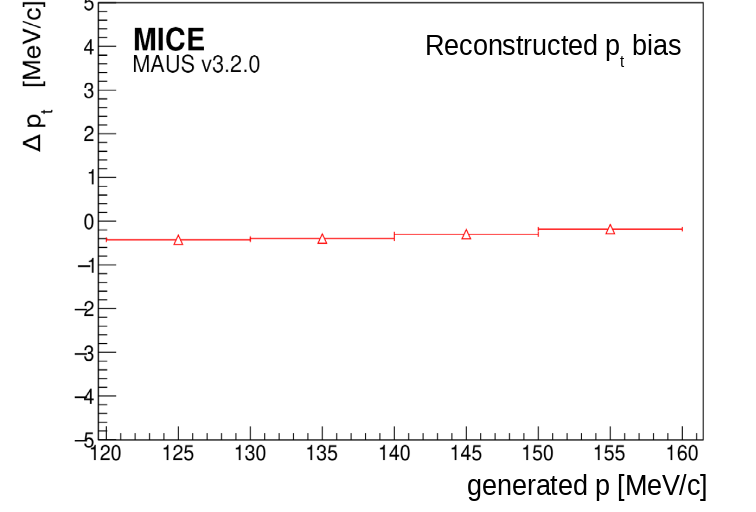
\includegraphics[width=0.49\textwidth]{upstream_pt_bias_p_logo.png}
    \end{tabular}
  \end{center}
  \caption{
    %Upstream tracker: from simulated data.
    Momentum reconstruction resolution (left) and bias
    (right) for the total momentum (top) and transverse momentum
    component (bottom) in the upstream tracker.
  }
  \label{trackers:performance:resolutions:up}
\end{figure}
\begin{figure}[htb]
  \begin{center}
    \begin{tabular}{cc}
      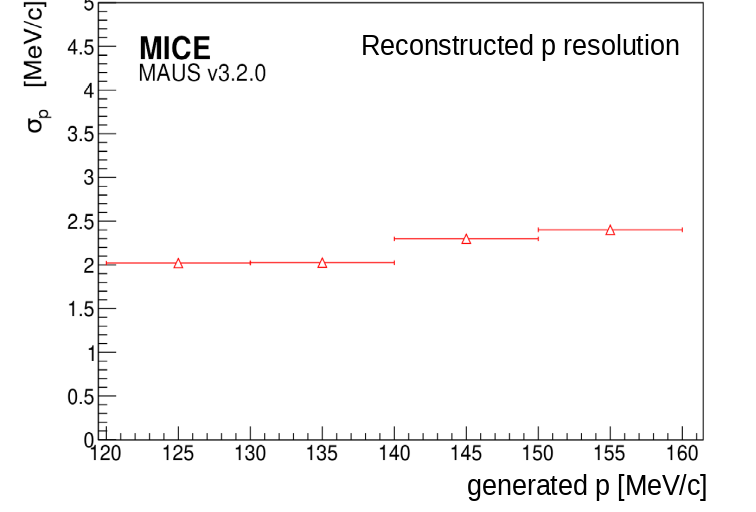
\includegraphics[width=0.49\textwidth]{downstream_p_resolution_p_logo.png} &	
      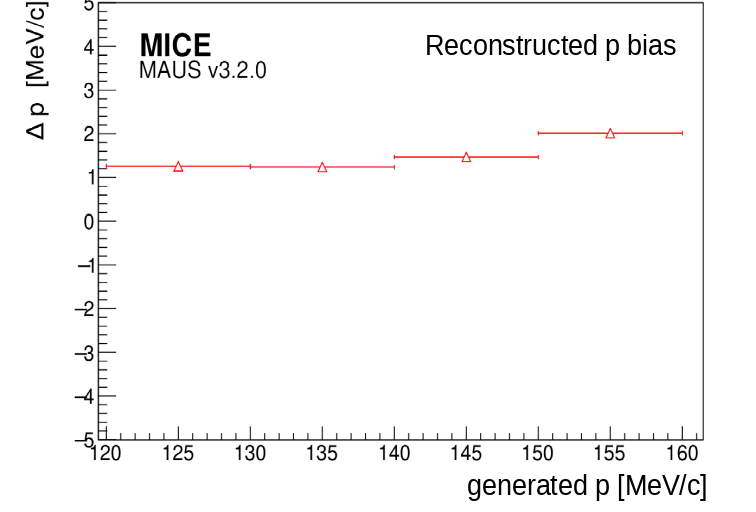
\includegraphics[width=0.49\textwidth]{downstream_p_bias_p_logo.png} \\
      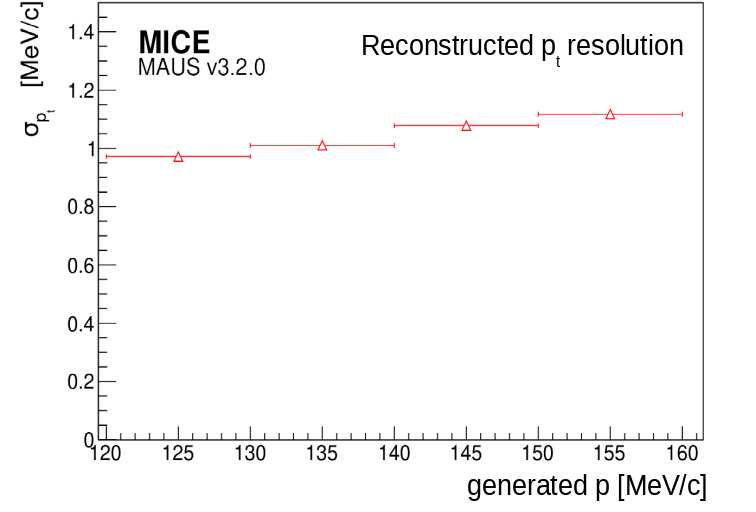
\includegraphics[width=0.49\textwidth]{downstream_pt_resolution_p_logo.png} &
      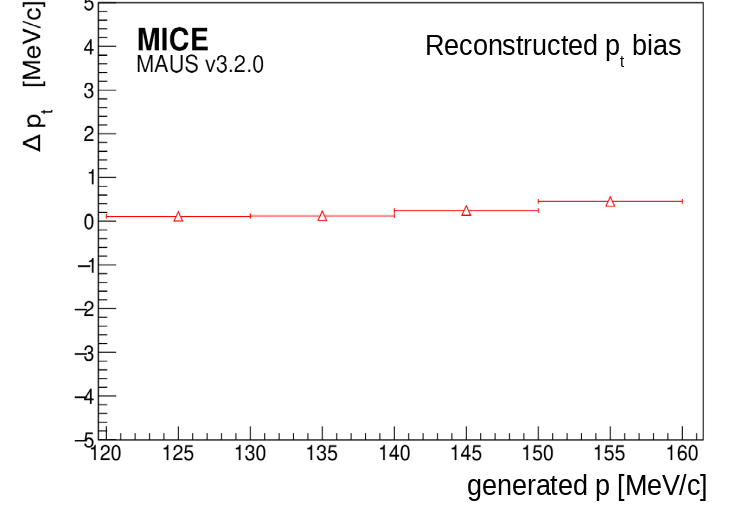
\includegraphics[width=0.49\textwidth]{downstream_pt_bias_p_logo.png}
    \end{tabular}
  \end{center}
  \caption{
    %Upstream tracker: from simulated data.
    Momentum reconstruction resolution (left) and
    bias (right) for the total momentum (top) and transverse
    momentum component (bottom) in the downstream tracker.
  }
  \label{trackers:performance:resolutions:down}
\end{figure}

%\graphicspath{{09-Detector-alignment/Figures/}}



\subsection{Beam-based detector alignment}
\label{SubSect:DA}

A beam-based alignment algorithm was developed to improve the
resolution on the position of the scintillating-fibre trackers
relative to the time-of-flight hodoscopes.
The starting point for the beam-based alignment was the geometrical
survey of the detectors in the MICE Hall which was performed using
laser geodesy. 
Survey monuments on the TOF frames were surveyed with respect to the
MICE Hall survey network.
The trackers had been dowelled in position in the bores of the
spectrometer solenoids.
The dowels were used to locate each tracker precisely with respect to the axis of the warm bore of its
solenoid.
The position of the trackers along the beam line was inferred from the
measurement of survey monuments mounted on the spectrometer-solenoid
cryostats outer jackets.
The beam-based alignment was used to determine the azimuthal
orientation of the trackers with a resolution of 6\,mrad/$\sqrt{N}$
and their position transverse to the beamline with a resolution of
20\,mm/$\sqrt{N}$, where $N$ is the number of tracks used in the
analysis~\cite{2018arXiv1805.06623T}. \\

\noindent\textbf{Analysis method} \\
\label{SubSect:DA_Analysis}
\noindent The position of each tracker in the MICE Hall coordinate
system was described using the location of its centre and a set of
three angles corresponding to rotation about the $x$ axis ($\alpha$),
the $y$ axis ($\beta$) and the $z$ axis ($\phi$).
The rotation of the tracker about the $z$ axis has a negligible effect
on the alignment since $\phi$ was determined precisely
at installation.
An initial estimate for the position of each tracker along the beamline
had been inferred from the survey.
The surveyed location of the TOFs was used as the reference for the
tracker alignment.
The line that joins the centre of TOF1 with the centre of TOF2 was
chosen as the reference axis.
A deviation from this axis was considered to be due to misalignment
of the trackers.
The alignment could not be determined on a single-particle basis due
to multiple Coulomb scattering in the absorber and other material
present on the beamline.
Therefore, the mean residuals in position ($x$ and $y$) and angle
($\alpha$ and $\beta$) of the trackers with respect to the TOF1--TOF2
axis were evaluated to determine the alignment constants.

Each TOF provided a single spacepoint in the Hall coordinate system.
In Hall coordinates, on average, the track reconstructed between
TOF1 and TOF2 should agree with the track reconstructed in each 
tracker, i.e. the mean residuals in $x, y, \alpha$, and $\beta$
should be zero. 
Applying this reasoning to the unknown offset and angles leads to a
system of equations for the four unknown
constants~\cite{2018arXiv1805.06623T}.
The measurement of four residual distributions per tracker yields the
alignment constants. 
The main source of bias was the scattering in the material between
TOF1 and TOF2.
If the beam was not perfectly centred, particles preferentially
scraped out on one side of the magnet bore, anisotropically truncating
the tail of the residual distribution. 
A fiducial cut was applied to the upstream sample in order to remove
this effect.

Data were recorded with the superconducting magnets turned off.
High momentum beams were used to reduce the RMS scattering angle and
to maximise transmission.   
Each data set was processed independently.
Figure~\ref{fig:runtorun} shows the alignment parameters determined for
each run during a specific data taking period.
The measurements are in good agreement with one another and show no
significant discrepancy: an agreement between the independent fits
guaranteed an unbiased measurement of the alignment constants.
The constant-fit $\chi^2/\text{ndf}$ was close to unity for each fit,
indicating that there were no additional sources of significant
uncertainty.
The optimal parameters are summarised in
table~\ref{tab:201701_constants}. 
\begin{table}
  \caption{
    Optimal alignment constants measured in the high-momentum straight-track data
    acquired during May 2017 (summarised from figure~\ref{fig:runtorun}).
    }
    \begin{center}
    \begin{tabular}{|l|c|c|c|c|}
  \hline
	& \textbf{x [mm]} & \textbf{y [mm]} & \textbf{$\alpha$ [mrad]} & \textbf{$\beta$ [mrad]} \\
	\hline
	\textbf{TKU} & $-0.032\pm0.094$ & $-1.538\pm0.095$ & $ 3.382\pm0.030$ & $0.412\pm0.029$ \\
	\textbf{TKD} & $-2.958\pm0.095$ & $ 2.921\pm0.096$ & $-0.036\pm0.030$ & $1.333\pm0.030$ \\
	\hline
    \end{tabular}
  \end{center}
  \label{tab:201701_constants}
\end{table}
\begin{figure}[htb]
  \begin{center}
    \begin{minipage}[b]{.45\textwidth}
      \begin{center}
        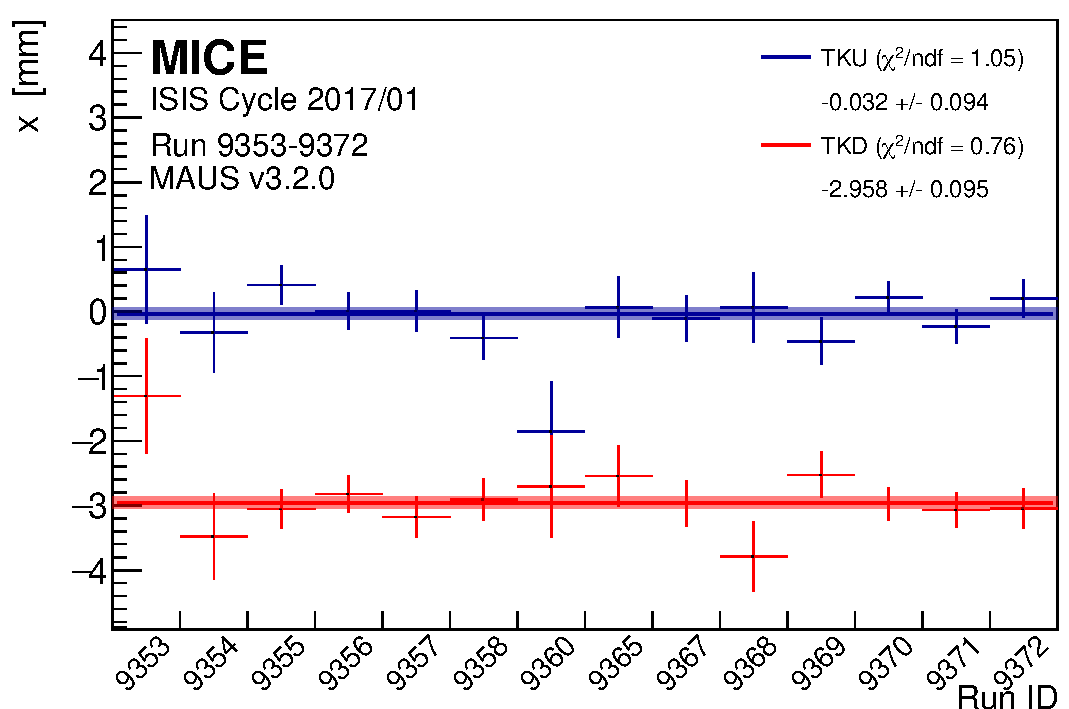
\includegraphics[width=\textwidth]{data_final/x_bestfit-edit.pdf}
      \end{center}
    \end{minipage}
    \hfill
    \begin{minipage}[b]{.45\textwidth}
      \begin{center}
        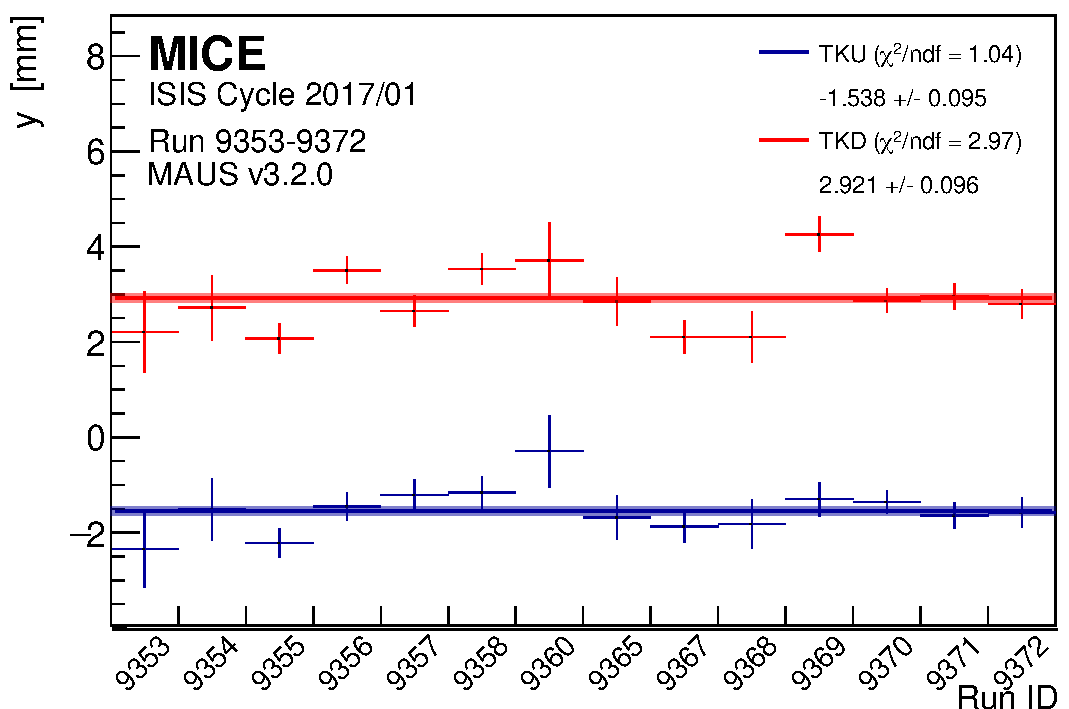
\includegraphics[width=\textwidth]{data_final/y_bestfit-edit.pdf}
      \end{center}
    \end{minipage}
    \begin{minipage}[b]{.45\textwidth}
      \begin{center}
        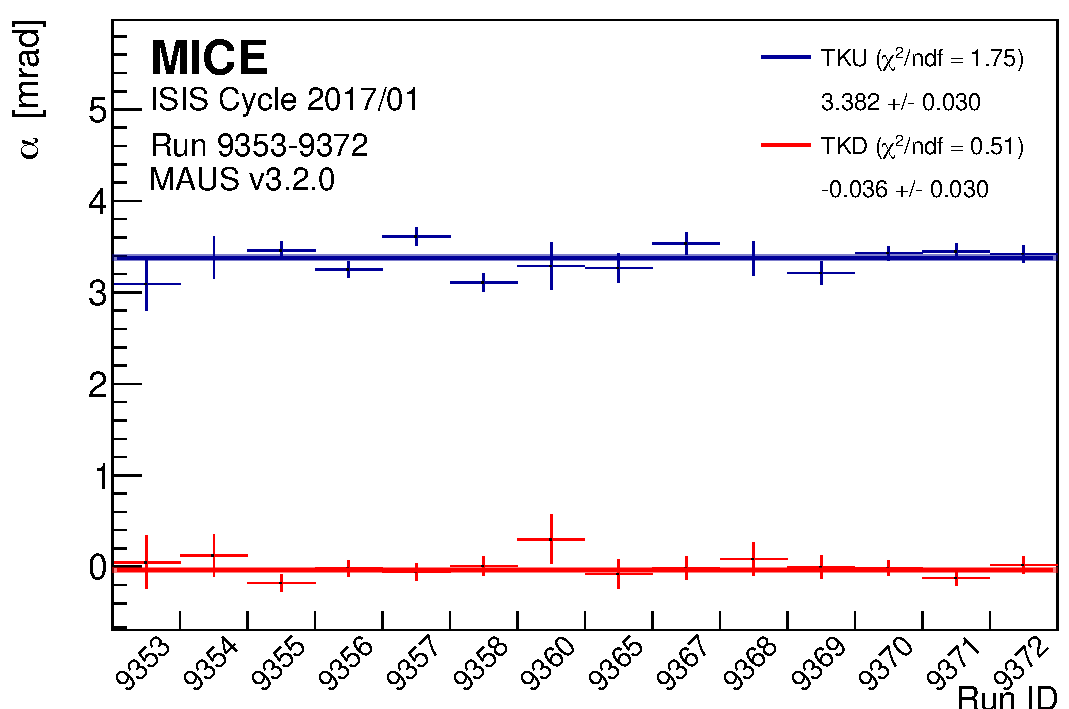
\includegraphics[width=\textwidth]{data_final/alpha_bestfit-edit.pdf}
      \end{center}
    \end{minipage}
    \hfill
    \begin{minipage}[b]{.45\textwidth}
      \begin{center}
        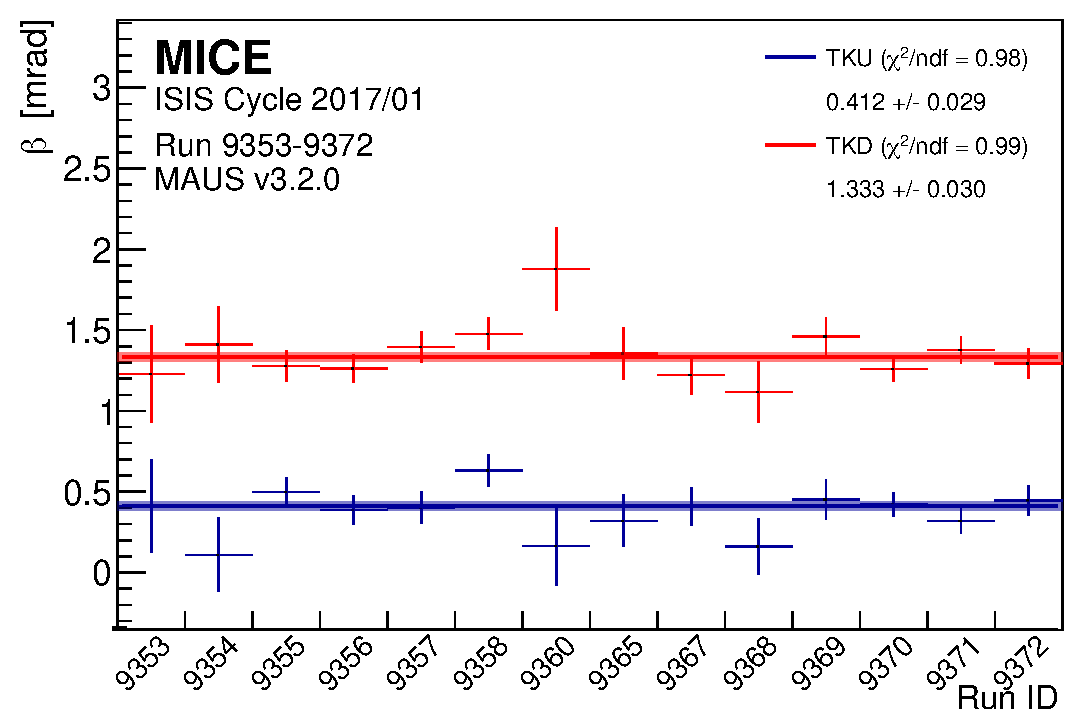
\includegraphics[width=\textwidth]{data_final/beta_bestfit-edit.pdf}
      \end{center}
    \end{minipage}
  \end{center}
  \caption{
    Consistency of the alignment algorithm results for upstream (blue) and downstream (red) trackers  across runs acquired during
    the 2017/01 ISIS user cycle. The quantities $x$, $y$, $\alpha$, and $\beta$ are defined in the text.
  }
  \label{fig:runtorun}
\end{figure}
